\documentclass[12pt]{article}
\usepackage[a4paper,margin=2.5cm]{geometry}
\usepackage{amsmath, amsfonts, amssymb, amsthm}
\usepackage{physics}
\usepackage{mathtools}
\usepackage{tikz}
\usetikzlibrary{decorations.pathreplacing}

\newcommand{\seg}[2]{\draw[line width=1.2pt] (#1,0)--(#2,0);}
\newcommand{\gris}[2]{\draw[line width=1.2pt,gray!55] (#1,0)--(#2,0);}
\title{Contra Ejemplos}
\author{Juan Rodríguez}
\date{}
\begin{document}
\maketitle
\section*{La intersección de un número finito o infinito de abiertos es un abierto}
Consideremos el conjunto \( A_n = \left( 1 -\frac{1}{n}, 2 + \frac{1}{n} \right) \) para \( n \in \mathbb{N} \). Cada \( A_n \) es un conjunto abierto en \( \mathbb{R} \). Ahora, consideremos la intersección infinita de estos conjuntos:
\[ \bigcap_{n=1}^{\infty} A_n = [1,2]. \]
El conjunto \( [1,2] \) es cerrado en \( \mathbb{R} \)
\section*{La unión de un número finito o infinito de cerrados es cerrado}
Consideremos el conjunto \( B_n = \left[ 1 +\frac{1}{n}, 2 - \frac{1}{n} \right] \) para \( n \in \mathbb{N} \). Cada \( B_n \) es un conjunto cerrado en \( \mathbb{R} \). Ahora, consideremos la unión infinita de estos conjuntos:
\[ \bigcup_{n=1}^{\infty} B_n = (1,2). \]
El conjunto \( (1,2) \) es abierto en \( \mathbb{R} \).
\section*{Si un espacio tiene una base no numerable, no puede tener otra numerable}
Consideremos el espacio topológico \( X = \mathbb{R} \) con la topología canónica, que tiene una base no numerable dada por \(\{(a,b) \in \mathbb{R}\}\). Pero, también podemos consider la base numerable \(\{(a,b) \in \mathbb{Q}\}\), que genera la misma topología.
\section*{En un espacio el mismo conjunto no puede ser a la vez abierto y cerrado}
Consideremos el espacio topológico \( X = \mathbb{R} \) con la topología Sorgenfrey, que tiene como base los intervalos de la forma \([a,b)\).
Tomemos el intervalo \([a, \infty)\).
Este conjunto es abierto porque se puede expresar como la unión de intervalos \([a, n+a)\).
\[
[a, \infty) = \bigcup_{n=1}^{\infty} [a, n+a)
\]
Por lo que su complemento \((-\infty, a)\) es cerrado.
Además, \((-\infty, a)\) también es abierto porque se puede expresar como la unión de intervalos \([-n, a)\).
\[(-\infty, a) = \bigcup_{n=1}^{\infty} [-n, a)\]
Por lo que su complemento \([a, \infty)\) es cerrado.
Así, el conjunto \([a, \infty)\) es a la vez abierto y cerrado en la topología Sorgenfrey.
\section*{Dos bases distintas no generan la misma topología}
Consideremos el espacio topológico \( X = \mathbb{R} \) con la topología del orden.
Dadas dos bases:
\begin{itemize}
    \item Base 1: \(\mathcal{B}_1 = \{((a,b), (c,d)) \mid (a,b) < (c,d)\}\)
    \item Base 2: \(\mathcal{B}_2 = \{((a,b), (a,d)) \mid b < d\}\)
\end{itemize}
Vemos que cualquier conjunto abierto generado por la base 1 puede ser expresado como una unión de conjuntos abiertos generados por la base 2. Por lo que \(\mathcal{B}_2 \subset \mathcal{B}_1\). Ambas bases generan la misma topología del orden en \( \mathbb{R}^2 \).
\section*{Dos distancias no equivalentes siempre generan topologías distintas}
Dos distancias no son equivales si:
\[
\forall k \quad \exists x,y \quad k \cdot d_1 < d_2 < d_1
\]
Tomemos las siguientes dos distancias en \( \mathbb{R}\):
\begin{itemize}
    \item \( d_1(x,y) = |x-y| \)
    \item \( d_2(x,y) = \arctan|x - y| \)
\end{itemize}
Podemos establecer que \(k \cdot |x-y| < \arctan|x - y| < \pi\) \\
Reducción al absurdo: 
\[
\forall k \quad |x-y| > \frac{\pi}{k} \rightarrow{x=2\pi, y=0} \rightarrow \frac{2\pi}{k} > \frac{\pi}{k} \quad \text{No se cumple } \forall k
\]
Por lo que \(d_1\) y \(d_2\) no son equivalentes. \\
Comprobamos ahora si ambas distancias generan la misma topología. \\
Sea \(x \in \mathbb{R}\) y \(r > 0\). Consideremos las bolas abiertas en cada distancia:
\[
B_{d_1}(x, r) = \{ y \in \mathbb{R} \mid |x - y| < r \}, \quad 
B_{d_2}(x, r) = \{ y \in \mathbb{R} \mid \arctan|x - y| < r \}.
\]
Como la función \(\arctan\) es estrictamente creciente y continua, se cumple que:
\[
\arctan|x - y| < r \quad \Leftrightarrow \quad |x - y| < \tan(r),
\]
por lo que:
\[
B_{d_2}(x, r) = B_{d_1}(x, \tan(r)).
\]
De forma análoga, dado que \(\tan\) y \(\arctan\) son funciones inversas, también se cumple:
\[
B_{d_1}(x, r) = B_{d_2}(x, \arctan(r)).
\]
Por lo tanto, cada bola abierta de una distancia puede expresarse como una bola abierta de la otra. \\
En consecuencia, ambas distancias generan la misma topología en \(\mathbb{R}\).
\section*{La función identidad siempre es continua, da igual la topología del espacio de
salida y la de llegada}
Consideremos el espacio topológico \( X = \mathbb{R} \) con la topología canónica y el espacio topológico \( Y = \mathbb{R} \) con la topología Sorgenfrey. La función identidad \( f: X \to Y \) está definida por \( f(x) = x \) para todo \( x \in \mathbb{R} \).
Para demostrar que \( f \) es continua, debemos verificar que la preimagen de cualquier conjunto abierto en \( Y \) es un conjunto abierto en \( X \). En la topología Sorgenfrey, una base de conjuntos abiertos está dada por los intervalos de la forma \([a, b)\) para \( a < b \).
Consideremos un conjunto abierto en \( Y \), \([1, 2)\). La preimagen de este conjunto es \[ f^{-1}([1, 2)) = [1, 2). \]
En la topología canónica de \( X \), el conjunto \([1, 2)\) no es abierto, por lo que la función identidad \( f \) no es continua.
\section*{Si una sucesión de funciones continuas converge a \(f(x)\) en cada punto, la función \(f(x)\) es continua}
Consideremos la sucesión de funciones \( f_n: \mathbb{R} \to \mathbb{R} \) definida por:
\[ f_n(x) = x^n \in [0,1]\]
Cada función \( f_n(x) \) es continua en \( \mathbb{R} \). Ahora, consideremos la función límite \( f(x) \) definida por:
\[ f(x) = \begin{cases} 
      0 & \text{si } 0 \leq x < 1 \\
      1 & \text{si } x = 1 
   \end{cases} \]
La función \( f(x) \) no es continua.
\section*{La distancia del supremo genera los mismos abiertos que la integral}
Consideremos el espacio de funciones continuas \(U=\{f(x)>0\}\) en el intervalo \([0,1]\). En la distancia del supremo, la bola abierta de radio \(r\) centrada en \(f(x)\) está dada por:
\[ B_{d_1}(f, r) = \{ g \in U \mid \|f - g\| < r \} \]
En la distancia de la integral, la bola abierta de radio \(r\) centrada en \(f(x)\) está dada por:
\[ B_{d_2}(f, r) = \{ g \in U \mid \int_0^1 |f(x) - g(x)| \, dx < r \} \]
Consideremos la función \(f(x) = 1\) y el radio \(r = 0.5\). La bola abierta en la distancia del supremo es:
\[ B_{d_1}(f, 0.5) = \{ g \in U \mid \|1 - g\| < 0.5 \} = \{ g \in U \mid |1 - g(x)| < 0.5 \text{ para todo } x \in [0,1] \} \]
Esto implica que \( g(x) \in (0.5, 1.5) \) para todo \( x \in [0,1] \).
Ahora, consideremos la bola abierta en la distancia de la integral:
\[ B_{d_2}(f, 0.5) = \{ g \in U \mid \int_0^1 |1 - g(x)| \, dx < 0.5 \} \]
Esto no garantiza que \( g(x) \) esté en el intervalo \( (0.5, 1.5) \) para todo \( x \in [0,1] \). Por ejemplo, una función \( g(x) \) que es \( 0 \) en la mitad del intervalo y \( 2 \) en la otra mitad cumple con la condición de la integral, pero no está en la bola abierta de la distancia del supremo.
Por lo tanto, las bolas abiertas generadas por la distancia del supremo y la distancia de la integral no coinciden, lo que implica que las topologías generadas por estas dos distancias son diferentes.

Nota: La distancia del supremo es más fina que la distancia de la integral.
\section*{La topología heredada de un espacio coincide siempre con la topología interior}
Contraejemplo: 
\[
A = ((0.5, 0.5); (0.5, 1)] \quad \text{en } [0,1] \times [0,1]
\]
En la heredada del plano es un abierto y en la del orden interno, no. \\

En la heredada en \([0,1] \times [0,1]\) es abierto porque 
\[
((0.5, 0.5); (0.5, 1)] = [0,1]^2 \cap ((0.5, 0), (0.5, 2))
\]

Sin embargo, en la del orden interno, \((0.5, 1)\) no es el máximo. 
El máximo es \((1,1)\), luego no puede ser cerrado, luego no es abierto. \\

Por tanto, la topología heredada del plano y la del orden interno no coinciden.
\section*{\(\operatorname{Int}(A\cup B) = \operatorname{Int}(A)\cup \operatorname{Int}(B)\)}
Contraejemplo en \(\mathbb{R}\): \\
\(A=\mathbb{Q}\), \(B=\mathbb{R}\setminus\mathbb{Q}\). \\
Entonces \(A\cup B=\mathbb{R}\) y \(\operatorname{Int}(A\cup B)=\mathbb{R}\),
mientras que \(\operatorname{Int}(A)=\operatorname{Int}(B)=\varnothing\).
\section*{\(\operatorname{Int}(\operatorname{Fr}(A))=\varnothing\)}
Contraejemplo en \(\mathbb{R}\): \\
Sea \(A=\mathbb{Q}\). Entonces \(\operatorname{Fr}(A)=\mathbb{R}\) y \(\operatorname{Int}(\operatorname{Fr}(A))=\mathbb{R} \neq \varnothing\).
\section*{La unión de clausuras es la clausura de la unión}
Contraejemplo:
\[
A_n = \left\{ \tfrac{1}{n} \right\}
\]
La clausura de la unión contiene el \(0\). Este contraejemplo solo es válido para una unión infinita. \\

\[
\bigcup \overline{A_n} \neq \overline{\bigcup A_n}
\]

\begin{itemize}
    \item \(\overline{A_n} = \left\{ \tfrac{1}{n} \right\} \Rightarrow \bigcup \overline{A_n} = \left\{ \tfrac{1}{n} : n \in \mathbb{N} \right\}\)
    \item \(\bigcup A_n = \left\{ \tfrac{1}{n} : n \in \mathbb{N} \right\} \Rightarrow \overline{\bigcup A_n} = \left\{ \tfrac{1}{n} : n \in \mathbb{N} \right\} \cup \{0\}\)
\end{itemize}

Por tanto, la igualdad no se cumple, ya que \(0\) pertenece a la clausura de la unión, pero no a la unión de las clausuras.
\section*{Sea cual sea la topología, una sucesión convergente siempre converge a un único punto}
Contraejemplo: 
\[
T = \{\emptyset, \{A\}, \{A,B\}, \{A,B,C\}\}
\]
en el conjunto \(X = \{A,B,C\}\). \\

Consideremos la sucesión constante:
\[
A, A, A, A, A, \dots
\]

Los abiertos que contienen a cada punto son:
\begin{itemize}
    \item \(A\): \(\{A\}, \{A,B\}, \{A,B,C\}\)
    \item \(B\): \(\{A,B\}, \{A,B,C\}\)
    \item \(C\): \(\{A,B,C\}\)
\end{itemize}

Como todos los términos de la sucesión son \(A\), se cumple que:
\[
A_n \in U \quad \forall n, \text{ para cualquier abierto } U \text{ que contenga a } A, B \text{ o } C.
\]

Por tanto, la sucesión \(A, A, A, \dots\) converge simultáneamente a \(A\), \(B\) y \(C\). \\
Esto demuestra que una sucesión puede tener más de un punto de convergencia dependiendo de la topología.
\section*{Un conjunto no numerable no puede ser no denso en ninguna parte}
Contraejemplo: el conjunto de Cantor \(C\subseteq[0,1]\).
\section*{Cantor: demostración gráfica de que no tiene interior}

\subsection*{Iteraciones de la construcción (se elimina siempre el tercio medio)}
\begin{center}
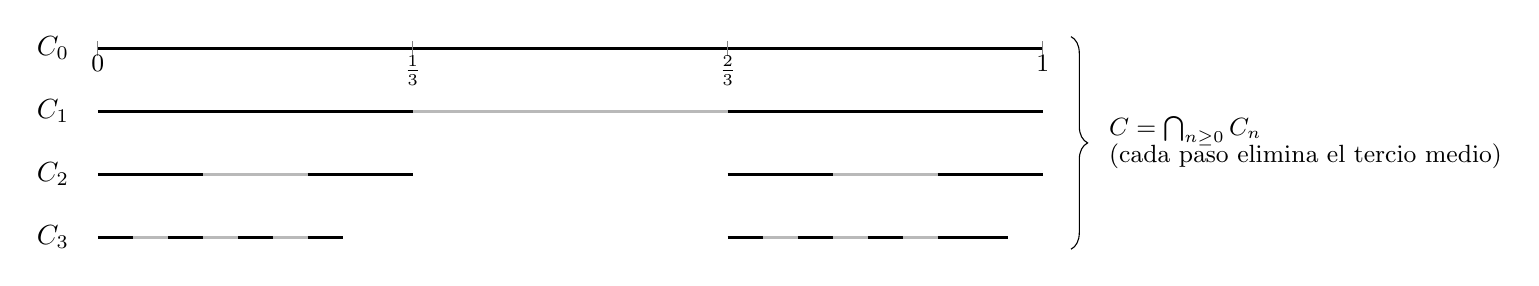
\begin{tikzpicture}[x=12cm,y=1cm]
  % Eje y labels
  \node[anchor=east] at (-0.02,0) {$C_0$};
  \node[anchor=east] at (-0.02,-0.8) {$C_1$};
  \node[anchor=east] at (-0.02,-1.6) {$C_2$};
  \node[anchor=east] at (-0.02,-2.4) {$C_3$};

  % C0
  \begin{scope}[shift={(0,0)}]
    \seg{0}{1}
    % marcas
    \draw[gray] (0,-0.1)--(0,0.1) node[below=2pt,black] {\small $0$};
    \draw[gray] (1/3,-0.1)--(1/3,0.1) node[below=2pt,black] {\small $\tfrac13$};
    \draw[gray] (2/3,-0.1)--(2/3,0.1) node[below=2pt,black] {\small $\tfrac23$};
    \draw[gray] (1,-0.1)--(1,0.1) node[below=2pt,black] {\small $1$};
  \end{scope}

  % C1
  \begin{scope}[shift={(0,-0.8)}]
    \seg{0}{1/3}
    \gris{1/3}{2/3}
    \seg{2/3}{1}
  \end{scope}

  % C2
  \begin{scope}[shift={(0,-1.6)}]
    \seg{0}{1/9}
    \gris{1/9}{2/9}
    \seg{2/9}{1/3}

    \seg{2/3}{7/9}
    \gris{7/9}{8/9}
    \seg{8/9}{1}
  \end{scope}

  % C3
  \begin{scope}[shift={(0,-2.4)}]
    % bloque izq
    \seg{0}{1/27}
    \gris{1/27}{2/27}
    \seg{2/27}{1/9}
    \gris{1/9}{4/27}
    \seg{4/27}{5/27}
    \gris{5/27}{2/9}
    \seg{2/9}{7/27}
    % bloque der
    \seg{2/3}{19/27}
    \gris{19/27}{20/27}
    \seg{20/27}{7/9}
    \gris{7/9}{22/27}
    \seg{22/27}{23/27}
    \gris{23/27}{8/9}
    \seg{8/9}{26/27}
  \end{scope}

  % llave y texto
  \draw[decorate,decoration={brace,amplitude=6pt}] (1.03,0.15) -- (1.03,-2.55);
  \node[align=left,anchor=west] at (1.06,-1.2)
  {\small $C=\bigcap_{n\ge0} C_n$\\[-2pt]
   \small (cada paso elimina el tercio medio)};
\end{tikzpicture}
\end{center}

\noindent
\textbf{Idea visible:} en cada escala aparecen \emph{huecos}. Ningún intervalo abierto logra
sobrevivir a todas las etapas, así que no puede haber un intervalo abierto
contenido en $C$.

\subsection*{Zoom local: en todo entorno hay un hueco}
\begin{center}
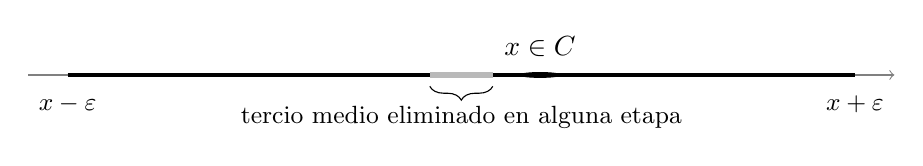
\begin{tikzpicture}[x=10cm,y=1.2cm]
  % intervalo del entorno
  \draw[gray,->] (-0.05,0)--(1.05,0);
  \draw (0,0) node[below=4pt] {\small $x-\varepsilon$};
  \draw (1,0) node[below=4pt] {\small $x+\varepsilon$};
  \seg{0}{1}

  % hueco en alguna etapa dentro del entorno
  \draw[very thick,white] (0.46,0)--(0.54,0);
  \draw[line width=2.2pt,gray!55] (0.46,0)--(0.54,0);
  \draw[decorate,decoration={brace,mirror,amplitude=5pt}] (0.46,-0.12)--(0.54,-0.12);
  \node at (0.5,-0.45) {\small tercio medio eliminado en alguna etapa};

  % marca x
  \draw[fill=black] (0.6,0) circle (0.025);
  \node[above=3pt] at (0.6,0) {$x\in C$};
\end{tikzpicture}
\end{center}

\noindent
\textbf{Conclusión gráfica:} cualquier intervalo $(x-\varepsilon,x+\varepsilon)$ contiene un
\emph{hueco} producido por la eliminación de un tercio en algún nivel.
Así, $(x-\varepsilon,x+\varepsilon)\nsubseteq C$. Como esto ocurre para todo $x\in C$
y todo $\varepsilon>0$, $C$ no tiene interior:
\[
\operatorname{int}(C)=\varnothing.
\]
Como además $C=\bigcap_{n\ge0}C_n$ es cerrado, se tiene
\[
\operatorname{int}(\overline{C})=\operatorname{int}(C)=\varnothing,
\]
y por tanto $C$ es \textbf{no denso en ninguna parte}.

\bigskip
\hrule
\bigskip

\paragraph{Cardinalidad de $C$.}
Cada punto de $C$ se codifica por una secuencia de dígitos ternarios usando sólo $\{0,2\}$.
Identificando $0\leftrightarrow 0$ y $2\leftrightarrow 1$, se obtiene una biyección con
las secuencias binarias $\{0,1\}^{\mathbb{N}}$ (no numerables). Gráficamente:
\[
\underbrace{0.\,{\color{blue}0}\,{\color{blue}2}\,{\color{blue}0}\,{\color{blue}2}\,\dots}_{\text{base }3}
\quad\longleftrightarrow\quad
\underbrace{0.\,{\color{blue}0}\,{\color{blue}1}\,{\color{blue}0}\,{\color{blue}1}\,\dots}_{\text{base }2}
\]
De aquí se deduce que $C$ es \textbf{no numerable}
\end{document}
